\chapter{3D Foot Placement Estimator and Gait Generation} % (fold)
\label{cha:simulations}

This chapter extends the Foot Placement Estimator (FPE) algorithm for 3D bipedal robots. The existing 2D FPE theory is reviewed in Section~\ref{sec:fpe_algorithm} and the significance of the FPE point on the ground is demonstrated through simulation. Section~\ref{sec:extension_to_3d} presents the method of extending the existing 2D theory for 3D space. The proposed algorithm selects a 2D plane in the chosen direction of motion and generates trajectories to produce a forward moving momentum along the plane. A whole body motion control framework coupled with a finite state machine is used to track the generated trajectories and form complete gait cycles. The toolchain described in the preivous chapter is used to generate dynamic simulations for the 14 DOF bipedal robot and the proposed extension to 3D is validated (Section~\ref{sec:simulations_and_results}).

\section{FPE Algorithm in 2D} % (fold)
\label{sec:fpe_algorithm}

Consider the standard compass biped model used widely in bipedal locomotion research today (shown in Figure \ref{fig:compass}). This simplified model is commonly used as the first step to reduce the complex dynamics to the two dimensional sagittal plane. The physical parameters are the mass $m$, inertia about the center of mass $I_{COM}$, leg lengths $L$ and leg separation angle $\beta$. Note that the angle $\theta_A$ is measured from the axis normal to the ground. 

\begin{figure}[!h]
	\centering
    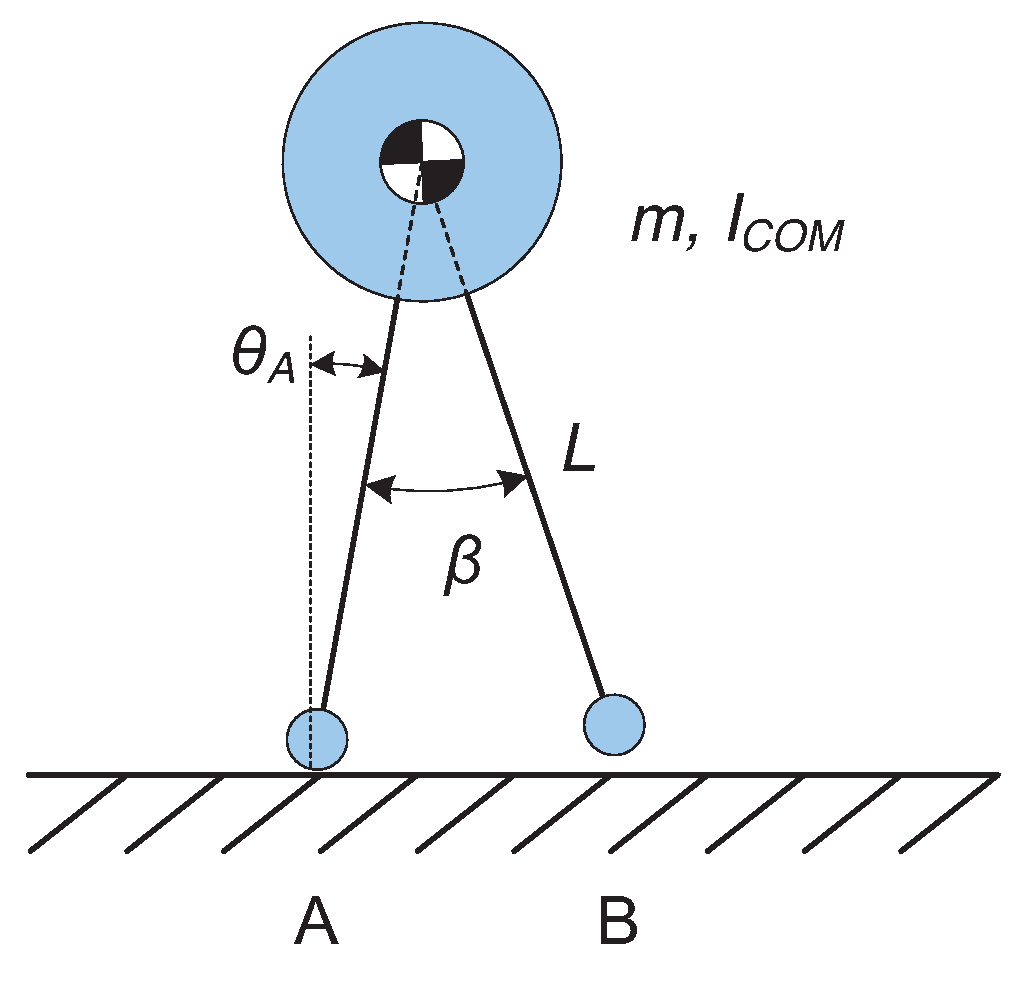
\includegraphics[scale=0.4]{fig/fpe/fig1.eps}
  	\caption{Standard compass biped model used for nonlinear analysis  and derivation of the FPE equation.}
	\label{fig:compass}
\end{figure}

Now consider this system at the moment when the swing leg comes into contact with the ground at point $B$ (the resulting behaviour is illustrated in Figure \ref{fig:prepost}). The following assumptions are made in reference to the behaviour of the system around the pre-impact and post-impact stages to simplify the model for further analysis \cite{Wight:2008vt}: 

\hrulefill

\begin{assumption}
	There is an instantaneous transfer of balance (i.e. the stance foot at point $A$ lifts up when the swing foot hits the ground at point $B$).  
\end{assumption}

\begin{assumption}
	The impact when the swing leg hits the ground at point $B$ is assumed to plastic. 
\end{assumption}

\begin{assumption}
	There is sufficient friction to prevent any slipping at the contact points. 
\end{assumption}

\begin{assumption}
	Gravity is assumed to be a non-impulsive force. 
\end{assumption}

\begin{assumption} \label{assump:betafix}
	The leg separation angle $\beta$ is fixed.
\end{assumption}

\begin{assumption} \label{assump:massless}
	The legs are massless and therefore do not significantly alter the dynamics of the system. 
\end{assumption}

\hrulefill

Note that assumption \ref{assump:betafix} implies that if both feet were to remain on the ground (i.e. double support phase), then by geometric symmetry about the normal, $\theta _A = \beta/2$. Equivalently, when leg $A$ is completely vertical, $\theta _A = 0$.

\begin{figure}[!h]
	\centering
    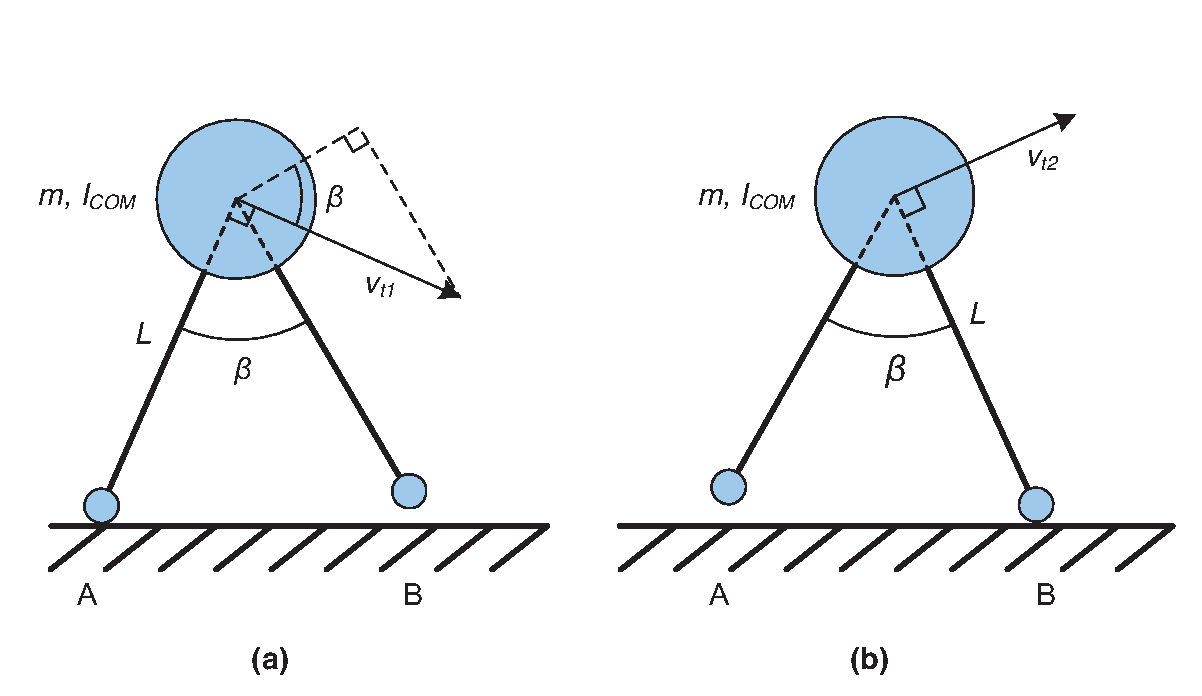
\includegraphics[scale=0.6]{fig/fpe/fig2.eps}
  	\caption{Compass biped model in the swing phase of the gait cycle in the (a) pre-impact and (b) post-impact configurations.}
	\label{fig:prepost}
\end{figure}

\subsection{Equations of Motion}

To formulate a state space representation of the biped, the equations of motion are derived as follows\footnote{Only key points of the derivation are summarized, for details on the full derivation of the FPE equation can be found in \cite{Wight:2008vt,Millard:2011vk}}. If the biped is treated as an inverted pendulum rotating about pivot point $A$ (i.e. configuration shown in Figure  \ref{fig:compass}), the equation of motion is found by applying Newton's second law:

\begin{equation}
	\begin{aligned}
		\sum {{\tau _A} = {I_A}} {{\ddot \theta }_A}
	\end{aligned}
\end{equation}

\begin{equation} \label{eq:compasseom1}
	\begin{aligned}
		{{\ddot \theta }_A} = \frac{{mgL\sin ({\theta _A})}}{{{I_{COM}} + m{L^2}}}
	\end{aligned}
\end{equation}

This equation is only valid while the inverted pendulum swings about point $A$ (i.e. pre-impact). When the swing leg comes in contact with the ground and based on the assumptions, point $B$ becomes the new pivot for inverted pendulum (post-impact). The motion of the post-impact system is now based on a different angular velocity (namely, $\dot{\theta}_B$). However, the assumptions 1-4 also relate the angular momentum of the system in the pre-impact stage (Figure \ref{fig:prepost}a) to the post-impact stage (Figure \ref{fig:prepost}b). Applying the conservation of angular momentum about point $B$, the post-impact angular velocity ($\dot{\theta}_B$) is a function of the pre-impact angular velocity ($\dot{\theta}_A$) \cite{Wight:2008vt} by the following: 

\begin{equation}
	\begin{aligned}
		{\dot \theta _B} = \frac{{({L^2}m\cos (\beta ) + {I_{COM}}){{\dot \theta }_A}}}{{{L^2}m + {I_{COM}}}}
	\end{aligned}
\end{equation}

While pivoting about point $B$, if the biped does not have enough momentum to swing all the way through then it simply rocks back until swing leg $A$ comes into contact with the ground. At this point, the equation of motion describing the system reverts back to \eqref{eq:compasseom1}. Given the geometric properties of the biped, it can be shown that the equation of motion about point $B$ is given by: 

\begin{equation} \label{eq:compasseom2}
	\begin{aligned}
		{\ddot \theta _B} = \frac{{mgL\sin ({\theta _B})}}{{{I_{COM}} + m{L^2}}} 
	\end{aligned}
\end{equation}

Together, $\theta _A$, $\theta _B$, along with its derivatives completely describe the motion of the compass biped. 

\subsection{Unified State Equations}
Assumption 5 imposes a geometric constraint which can be used to combine the variables which completely define the motion. At the instant of impact, the angles $\theta _A$ and $\theta _B$ can be expressed as: 

\begin{equation}
	\begin{aligned}
		{\theta _A} = \theta  + \frac{\beta}{2} \\
		{\theta _B} = \theta  - \frac{\beta}{2}
	\end{aligned}
\end{equation}

Where the angles $\theta _A$, $\theta _B$, $\theta$ and $\beta$ are shown on Figure \ref{fig:unified}. The single (unified) variable $\theta$ can be formed by rearranging the equations of motion described in terms of $\theta _A$ and $\theta _B$: 

\begin{subnumcases}{\ddot{\theta}=\label{eq:unifiedeom}}
	\frac{{mgL\sin (\theta  + \beta /2)}}{{{I_{COM}} + m{L^2}}} & $\theta < 0$ \\
	\frac{{mgL\sin (\theta  - \beta /2)}}{{{I_{COM}} + m{L^2}}} & $\theta > 0$ \\
	\frac{{mgL\sin (\theta  + \beta /2)}}{{{I_{COM}} + m{L^2}}} & $\theta = 0$, $\dot{\theta} > 0$ \\
	\frac{{mgL\sin (\theta  - \beta /2)}}{{{I_{COM}} + m{L^2}}} & $\theta = 0$, $\dot{\theta} < 0$ \\
	\quad \quad \quad \quad 0 & $\theta = 0$, $\dot{\theta} = 0$
\end{subnumcases}

The system defined by \eqref{eq:unifiedeom} is used to investigate stability and subsequently derive the FPE equation. For future reference, define the following function to represent conditional equation of motion corresponding to a region of the state space (defined by $\theta$ and $\dot{\theta}$): 

\begin{equation}  
	\begin{aligned}
		\ddot{\theta} \eqdef F(\theta, \dot{\theta})
	\end{aligned}
\end{equation}

\begin{figure}[!t]
	\centering
    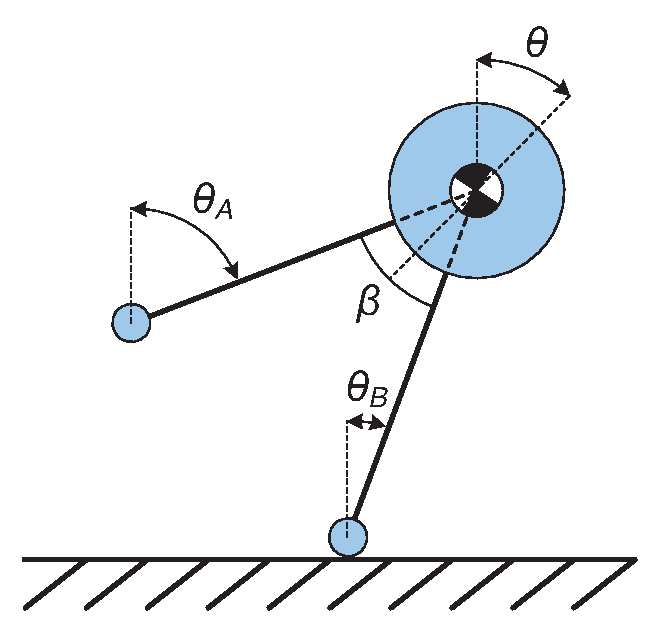
\includegraphics[scale=0.7]{fig/fpe/fig3.eps} 
  	\caption{Unified variable $\theta$ used to simplify the analysis. It is easily observed that $\theta_A = \theta  + \beta /2$ and $\theta_B = \theta  - \beta /2$}.
	\label{fig:unified}
\end{figure}

This unified variable is used to form a state space representation with the states as $\theta$ and $\dot{\theta}$: 

\begin{equation} \label{ss}
	\begin{aligned}
				\begin{gathered}
  			\dot{\Theta} = \left[ {\begin{array}{*{20}{c}}
  {\dot \theta } \\ 
  {F(\theta, \dot{\theta})} 
							   \end{array}} \right]
		\end{gathered}
	\end{aligned}
\end{equation}

\subsection{Conditions for Stability}
The notion of stability (or lack there of) is explicitly defined by \cite{Wight:2008vt} as follows: 

\hrulefill

\begin{definition} \label{def:fallen}
	The biped has fallen if $\dot{\theta} = 0$ and any other point other than the feet is in contact with the ground. 
\end{definition}

\begin{definition} \label{def:balanced}
	The biped is balanced if $\dot{\theta} = 0$ and it has not fallen. 
\end{definition}

\begin{definition} \label{def:stable}
	The biped has stable if for a given set of initial conditions and no further energy input to the system, the biped eventually comes to a rest in an upright position. Once at rest, a sufficiently small, impulsive, nonzero external disturbance to the biped should result in motion that will eventually return to the same stable, balanced position. 
\end{definition}

\hrulefill

\begin{figure*}[!t]
	\begin{equation} \label{eq:fpe}
	\begin{aligned}
		\frac{{{{\left[ {mh({v_x}\cos \phi  + {v_y}\sin \phi )\cos \phi  + {I_{COM}}{{\dot \theta }_1}{{\cos }^2}\phi } \right]}^2}}}{{m{h^2} + {I_{COM}}{{\cos }^2}\phi }} + 2mgh\cos \phi (\cos \phi  - 1) = 0
	\end{aligned}
	\end{equation}
	\\ 
	\hrulefill
\end{figure*}

The only physical configuration that can be achieved by definition \ref{def:balanced} is if the biped is double support phase. This implies that being balanced is mathematically equivalent to the system $\dot{\Theta}$ remaining at its stable equilibrium at the origin. The second part of definition \ref{def:stable} implies that stability in the physical sense is equivalent to the origin of system $\dot{\Theta}$ being asymptotically stable (since the biped should return to the same balanced position after small enough perturbations.

Thus, it is possible to determine the conditions for which the biped is stable if it it can be shown that the origin of \eqref{ss} is asymptotically stable. To this end, a Lyapunov function candidate based on the energy of the system ($U = T + V$) with an offset in potential energy is chosen to show asymptotic stability. For example, for the first equation of motion represented by \eqref{eq:unifiedeom} for $\theta < 0$: 

\begin{equation}
	\begin{aligned}
		V(\Theta) &= {\frac{1}{2}({I_{COM}} + m{L^2}){\dot \theta ^2} + mg(h - {h_{datum}})}	
		\end{aligned}
\end{equation}

Where $h =\cos (\theta+\beta/2) $ and $h_{datum} = \cos (\beta/2)$. The Lyapunov candidate is positive definite if $-\beta/2 < \theta < \beta/2$ with the following $\dot{V}(\Theta)$: 

\begin{equation}
	\begin{aligned}
			\dot{V}(\Theta) &= ({I_{COM}} + m{L^2}){\dot \theta ^2}F(\theta ,\dot \theta ) - mgL\sin (\theta  + \beta /2)\dot \theta
	\end{aligned}
\end{equation}

Analyzing the behaviour of $\dot{V}(\Theta)$ involves looking at each region of the state space specified by \eqref{eq:unifiedeom} and investigating the behaviour within the local region. In summary, $\dot{V}(\Theta) = 0$ for the cases where $\theta \not= 0$  (i.e. \ref{eq:unifiedeom}a and \ref{eq:unifiedeom}b) and is negative definite when $\theta = 0$, $\dot{\theta} \not= 0$ (i.e. \ref{eq:unifiedeom}c and \ref{eq:unifiedeom}d). Furthermore, the equilibrium point is the largest invariant set in: 
\[E = \left\{ {\Theta |\dot V(\Theta ) = 0} \right\}\]
Thus, by the Barbashin-Krasovskii-LaSalle principle it is shown that origin of $\dot{\Theta}$ is locally asymptotically stable in the sense of Lyapunov. In order to determine which initial conditions will exhibit a decaying orbit towards the origin, the exact boundaries of the local stability is obtained by analyzing the behaviour of the total system energy with different initial conditions. 

\subsection{Computing the FPE Angle} % (fold)
\label{sub:computing_the_fpe_angle}
Given that the system is asymptotically stable and the exact boundaries of the local stability are defined, it is possible to determine whether a specific location in the state space is stable in the sense of definition \ref{def:stable}. However, the goal for FPE is to determine where the foot must be placed in order to restore stability, so the knowledge of the local stability is used to reformulate the problem. 

To this end, the approach described in \cite{Wight:2008vt} introduces a parameter known as the FPE angle ($\phi$). The projection from the COM at an this angle $\phi$ to the ground surface provides the location of where the foot would need to be placed in order to restore stability to the unbalanced system. The actual solution to \eqref{eq:fpe} yields the FPE angle $\phi$, which can be obtained by using numerical techniques for solving non-linear equations. In essence, the FPE angle $\phi$ specifies the configuration system to enter/remain inside the locally stable region of $\dot{\Theta}$ if it were to step in the \textit{next} instant. By continuously tracking this angle while the biped is about to land the swing foot, the angle $\phi$ eventually converges to $\beta/2$ prior to impact.

Note that so far, the simple compass biped model used made several assumptions which are now lifted. The leg separation angle $\beta$ is no longer a fixed value throughout the whole gait cycle. Instead, by assumption \ref{assump:massless} that the legs are massless (and therefore they do not alter the dynamics of the system), the value of $\beta$ can vary while the swing leg is being brought over to the contact point for the subsequent step. The solution to the FPE equation requires only that the leg length $L$ and angle $\beta$ are fixed at the instant of impact. Simply put, the compass biped model used in the derivation thus far only represents how a real biped looks when an impact occurs. During the swing phase, an arbitrary and more realistic model of the biped looks like as shown in Figure \ref{fig:phi}, where the angle $\phi$, projection from the COM and the FPE location on the ground plane are visualized. 

\begin{figure}[h]
	\centering
    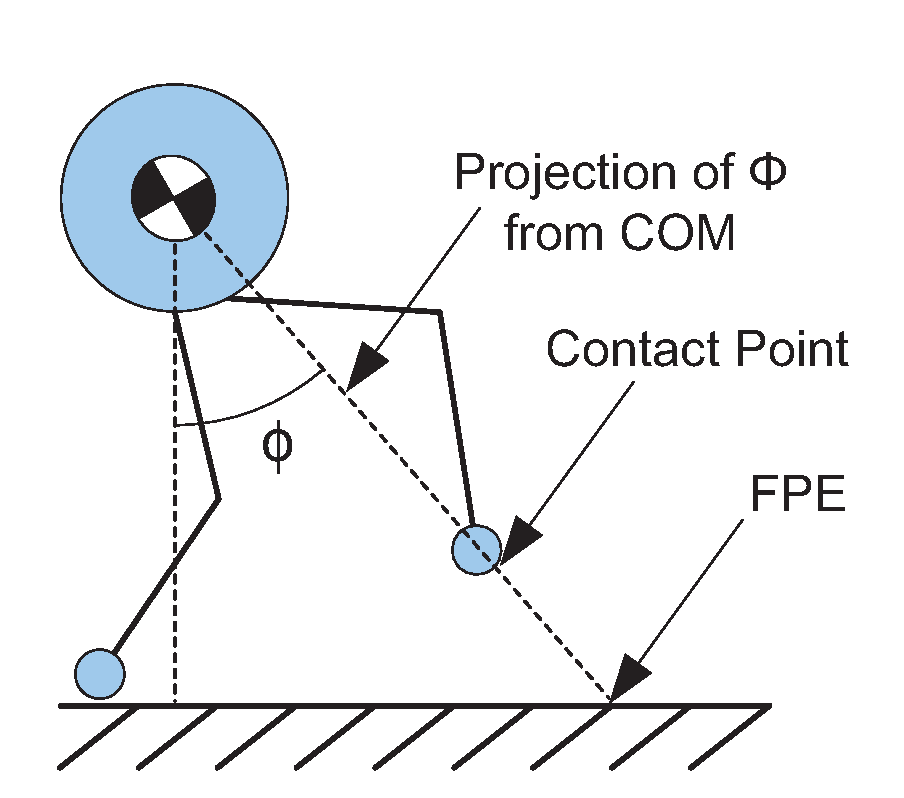
\includegraphics[scale=0.6]{fig/fpe/fig5.eps}
  	\caption{Graphical representation of the solution to the FPE equation for arbitrary robot configurations.}
	\label{fig:phi}
\end{figure}

% subsection computing_the_fpe_angle (end)

\subsection{Stability Analysis} % (fold)
\label{sub:overstepping_understepping_simulation}

In order to show that stepping on the FPE point can restore stability to an unbalanced system, the unified state space model was implemented in simulation along with a numerical solver for the nonlinear FPE equation \eqref{eq:fpe}. Three experiments were devised to analyze the behaviour of the system when the swing foot steps exactly on, behind and ahead of the FPE location obtained from the solver. These three cases are labelled perfect, under and over stepping, respectively. The simulations assume arbitrary physical parameters for $m$, $I_{COM}$, etc. The compass biped model with the single state variable is simulated to illustrate the effects of overstepping and under stepping. The leg separation angle $\beta$ is held constant and no energy is lost upon impact. 

\begin{figure}[!h]
	\begin{center}
	\subfigure{\includegraphics[scale=0.43]{fig/simulations/perfectsteppingtime.eps}}
	\subfigure{\includegraphics[scale=0.43]{fig/simulations/perfectsteppingphase.eps}}
	\end{center}
  	\caption{Time evolution and state trajectories for perfect stepping (i.e. foot lands extactly on the FPE point)}
	\label{sim:perfect}
\end{figure}

The results of the perfect stepping case shown in Figure \ref{sim:perfect} validate the efficacy of the FPE point on the ground. Starting from an unstable configuration, the simple biped model exhibits stability (i.e. rocking back and forth) due to no energy loss in the system by assumption. For a real physical biped, the energy losses experienced during impact would produce a decaying orbit towards the origin due to the asymptotic stability of the system within this local region. 

\begin{figure}[!h]
	\begin{center}
	\subfigure{\includegraphics[scale=0.43]{fig/simulations/understeppingtime.eps}}
	\subfigure{\includegraphics[scale=0.43]{fig/simulations/understeppingphase.eps}}
	\end{center}
  	\caption{Time evolution and state trajectories for under stepping (i.e. foot lands behind FPE point)}
	\label{sim:under}
\end{figure}

In the under stepping case, the swing foot lands short of the FPE location on the ground. This behaviour results in an excessive energy and momentum which causes the biped to eventually fall over. Starting from the same initial conditions presented in the perfect stepping case, the results of understepping is shown in Figure \ref{sim:under}. The time evolution and state trajectories exhibit unstable behaviour, further validating the results presented in \cite{Wight:2008ii}. 

\begin{figure}[!h]
	\begin{center}
	\subfigure{\includegraphics[scale=0.43]{fig/simulations/oversteppingtime.eps}}
	\subfigure{\includegraphics[scale=0.43]{fig/simulations/oversteppingphase.eps}}
	\end{center}
  	\caption{Time evolution and state trajectories for over stepping (i.e. foot lands in front of FPE point)}
	\label{sim:over}
\end{figure}

Lastly, the results of overstepping with the same initial conditions is presented in Figure \ref{sim:over}. As expected, if the swing foot lands ahead of the FPE location, the system enters a stable orbit where the biped rocks back and forth. As mentioned previously, the energy losses experienced during impact for a real biped would cause this closed orbit to decay and eventually reach the equilibrium due to local asymptotic stability. 

% subsection overstepping_understepping_simulation (end)

\subsection{Forming Complete Gait Cycles} % (fold)
\label{sub:gait_cycles}
Wight used the FPE concept to develop full gait cycles using simple linear control techniques and a state machine \cite{Wight:2008vt}. Gait is initiated by destabilizing the robot in the desired direction of movement (forward or backward). Once destabilized, the FPE equation is solved numerically to obtain the FPE angle $\phi$, which is used to provide the desired trajectory for the swing foot. 

\begin{figure}[!h]
	\centering
    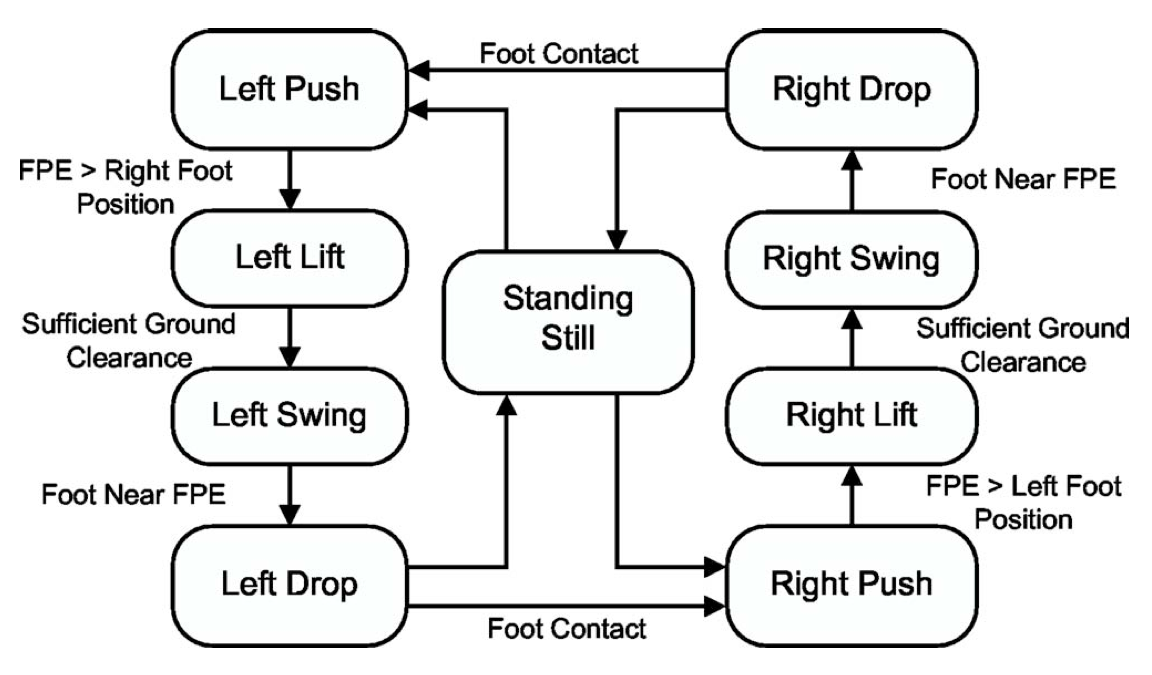
\includegraphics[scale=0.4]{fig/simulations/fpestatemachine.png}
  	\caption{A simple state machine used in conjunction with the FPE algorithm to form complete gait cycles}.
	\label{fig:statemachine}
\end{figure}

If continued forward progress is desired, the foot is commanded to precede the FPE. If no further forward progress is needed, the foot is commanded to the FPE. The desired trajectory is resolved to joint angles using inverse kinematics and implemented via joint level PD controllers. The complete state machine is shown in Figure~\ref{fig:statemachine}. Due to symmetry, the states in Figure~\ref{fig:statemachine} can be reduced to \textbf{STAND}, \textbf{PUSH}, \textbf{LIFT}, \textbf{SWING} and \textbf{DROP}. For the remainder of this paper, the sequence of state transitions from \textbf{PUSH} to \textbf{DROP} is referred to as the step cycle.
% subsection forming_complete_gait_cycles (end)


% section fpe_2D (end)

\section{FPE Extension to 3D} % (fold)
\label{sec:extension_to_3d}

In order to extend the FPE approach to the 3D case, the concept of generating complete gait cycles described in Section~\ref{sub:gait_cycles} is revisted. The primary goal of the first three states in each step cycle (\textbf{PUSH}, \textbf{LIFT} and \textbf{SWING}) is to force the biped into an unstable configuration so that the FPE algorithm can be used to regain stability in the terminal state (\textbf{DROP}).

To extend the 2D algorithm to the general 3D case, we begin by selecting a suitable plane in 3D space as the sagittal plane. The off-sagittal plane is perpendicular to the sagittal plane and the ground.  In the proposed approach, the goal of each step cycle is to control the motion of a 3D bipedal robot to generate a forward moving momentum \emph{along} the selected sagittal plane. Upon entering the terminal state, the FPE equation (\ref{eq:fpe}) is solved on the selected plane to determine the swing foot placement and ultimately regain stability. Unlike the 2D case, consider a 3D bipedal robot with finite foot length and width rather than a biped with point feet as demonstrated in \cite{Wight:2008vt}. The larger size of the region of support increases robustness to these approximation errors. 

The remainder of this thesis assumes a 3D bipedal robot with $n$ actuated degrees of freedom (DOF) and $n+6$ generalized coordinates defined by (\ref{eq:eom1}). 

\subsection{Sagittal Plane} % (fold)
\label{sub:sagittal_plane}
To select an appropriate sagittal plane for a 3D bipedal robot, a vertical plane which lies between the current position of the stance foot and the desired direction of motion is chosen. For a 3D biped walking in a forward motion, this plane is chosen as the the vertical plane passing through the midpoint between the hips and parallel to the direction of forward progress. For side-stepping motion, the coronal plane through the stance foot in the direction of the side step is chosen as the sagittal plane.

The motion of the biped is controlled based on the selected plane for the duration of the step cycle. During gait initiation, the lines from the COM to the contact points are of length $L$, and the leg separation angle is $\beta$ (similar to the planar case). If the motion of the biped is constrained along this plane, the FPE angle $\phi$ can be used to determine foot placement to regain stability. The parameters required to compute the 2D FPE along the plane are computed accordingly. That is, the inertia tensor of each link is rotated to obtain the appropriate $I_{COM}$ along the selected sagittal plane.

Upon impact, the angle $\phi$ converges to $\beta/2$ and a new sagittal plane can be selected for the subsequent step cycle prior to the swing leg entering the \textbf{PUSH} state. Once selected, the stance foot is rotated for alignment and swing leg trajectories can be generated along the plane. By selecting a plane between the current and desired directions of motion, this approach can achieve turning with each step.

% subsection sagittal_plane (end)

\subsection{Trajectory Generation} % (fold)
\label{sub:trajectory_generation}
Once the sagittal plane has been identified at the beginning of each step cycle, appropriate task space trajectories must be generated for the COM ($x_{COM}$) and the swing foot ($x_{SWING}$).

In the 2D case, the main goal of the initial states \textbf{PUSH}, \textbf{LIFT} and \textbf{SWING} was to achieve enough forward motion to destabilize the biped. In the 3D case, the robot must also remain stable in the off-sagittal plane while achieving the desired sagittal plane motion. If the ZMP leaves the region of support formed by the stance foot as the swing foot is lifted, the biped begins to fall in the off-sagittal plane and the solution to the 2D FPE equation is insufficient to maintain stable gait. To ensure both forward progress and off-sagittal plane stability, the generated trajectories for $x_{COM}$ are shown in Figure~\ref{fig:comtraj3d}. \\

\textbf{PUSH}: $x_{COM}$ is moved above the leading stance foot to maintain stability in the off-sagittal and sagittal planes.

\textbf{LIFT}: $x_{COM}$ is held at its current location (above stance foot) while the swing foot is lifted from the ground to achieve sufficient clearance.

\textbf{SWING}: $x_{COM}$ is held in place until the swing foot is aligned with the stance foot in the off-sagittal plane. At this point the $x_{COM}$ is deliberately pushed outside the region of support in the sagittal plane direction. \\

\begin{figure}[!h]
	\centering
    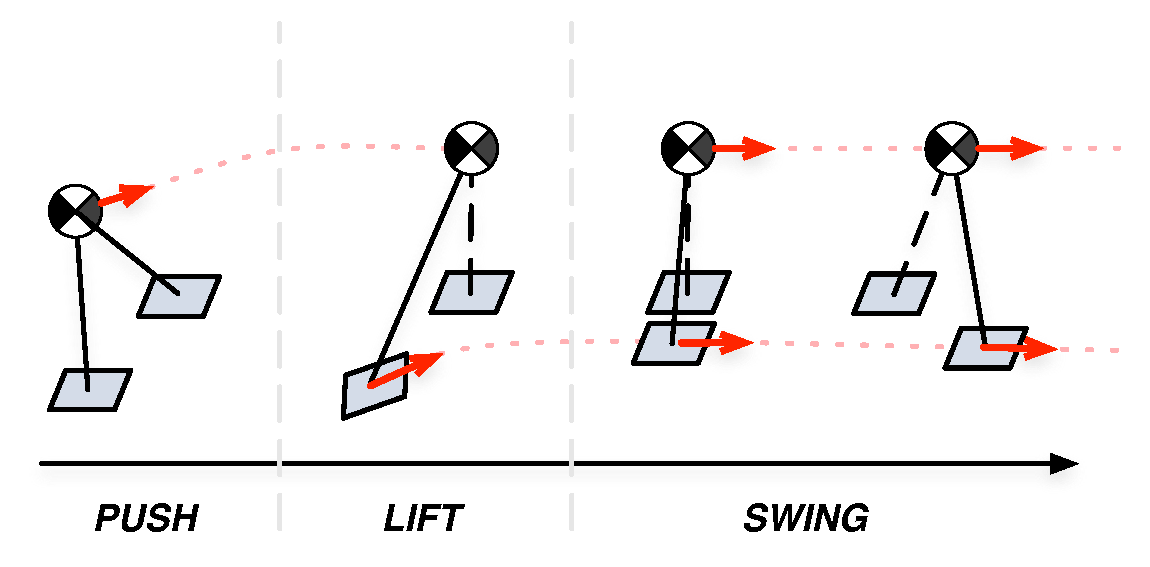
\includegraphics[scale=0.7]{fig/fpe/comtraj3d.eps} 
  	\caption{Trajectory for $x_{COM}$ to ensure forward progress and off-sagittal stability for 3D FPE. \Incomplete}
	\label{fig:comtraj3d}
\end{figure}


A similar approach is used to generate trajectories for $x_{SWING}$ to achieve the desired behaviour of generating enough momentum to destabilize the biped in the sagittal plane while maintaining stability in the off-sagittal plane. Trajectories for $x_{SWING}$ (illustrated in Figure~\ref{fig:swingfoottraj}) are always computed to align with the sagittal plane formed by the stance foot at the start of the step cycle. This ensures that the solution to the 2D FPE equation remains valid as the \textbf{DROP} state is entered. \\

\textbf{PUSH}: $x_{SWING}$ is held in place as the $x_{COM}$ trajectory is tracked.

\textbf{LIFT}: $x_{SWING}$ follows a ramped trajectory to simultaneously raise the foot off the ground and move it forward in the sagittal plane.

\textbf{SWING}: $x_{SWING}$ follows a straight line trajectory at a specific ground clearance (shown as $h_{LIFT}$ on Figure~\ref{fig:swingfoottraj}) until it reaches the FPE angle $\phi$. \\

\begin{figure}[!h]
	\centering
    \includegraphics[scale=0.6]{fig/fpe/swingfoottraj.eps} 
  	\caption{Trajectory for $x_{SWING}$ along the selected (sagittal) $xz$-plane for 3D FPE. \Incomplete}
	\label{fig:swingfoottraj}
\end{figure}

The ramp trajectory used to raise the swing foot during \textbf{LIFT} should be parameterized in terms of the velocity of the FPE point so that this state transitions faster in the event of larger disturbances (since the biped would have a shorter amount of time to swing the foot over and catch itself).

Depending on the supervisory control mode (i.e. \textbf{WALK} or \textbf{STAND}), the swing leg trajectory can be adjusted to implicitly achieve a desired goal. During \textbf{WALK} mode, the swing foot trajectory tracks a point on the ground slightly behind the FPE point. This under stepping behaviour results in the biped having enough forward moving momentum when the swing foot comes in contact with the ground such that the biped is unstable. As a result, the FPE point is continuously moving forward causing the state machine to transition into the opposing foot's \textbf{LIFT} state upon contact. In the \textbf{STAND} mode, the swing foot trajectory is adjusted to overstep the FPE point so that the biped comes to a stop following this step.

% subsection task_space_trajectory_generation (end)

\subsection{Control Strategy} % (fold)
\label{sub:control_strategy}

A hybrid control strategy is used to simultaneously maintain stability in the off-sagittal plane, achieve sufficient forward momentum along a selected sagittal plane and ultimately track the FPE location to regain stability by taking a step. Similar to the approach presented in \cite{Wight:2008vt}, this approach uses a state machine to transition through the step sequence with each state having a local controller.

During the initial states of the step cycle, whole body motion control is used to track the $x_{COM}$ and $x_{SWING}$ trajectories described in  Section~\ref{sub:trajectory_generation}. To generate the corresponding joint level trajectories, the Jacobian matrix is used to map between the task space and the joint space velocities:

\begin{IEEEeqnarray}{rCl}
	\label{eq:jmap}
	J & = & \begin{bmatrix} \partial q_{act} & \partial x_{base} \\ \end{bmatrix}_{m \times (n+6)}
\end{IEEEeqnarray}

A prioritized task space control scheme is used to generate joint level trajectories which simultaneously achieve state goals while satisfying the highest priority constraint (i.e. holding the $x_{COM}$ position). The state-dependent joint level trajectories can be computed by projecting the lower priority task space goals onto the null space of higher priorities:

\begin{eqnarray}
	\label{eq:priori}
	\dot{q}_{ref} = S(J_{H}^{\#} \dot{x}_{H} + N_{H} J_{L}^{\#} \dot{x}_{L})
\end{eqnarray}

Where, $S = \begin{bmatrix} I_{n \times n} & 0_{n \times 6} \\ \end{bmatrix}$ is the actuator selection matrix for (\ref{eq:gentau}), $J^{\#}$ is the psuedoinverse of the Jacobian $J$, $\dot{q}_{ref}$ is the reference joint velocity, and $\dot{x}_H$ and $dot{x}_L$ are the high and low priority task space velocities, respectively. $J_{H}$ are $J_{L}$ are the corresponding high and low priority Jacobians, and $N_{H} = I - J_{H}^{\#} J_{H}$ is the null space projection matrix. The reference joint velocities are integrated to obtain the reference command signal to be tracked by high gain local PD controllers. The specific prioritization of each state is discussed in Section~\ref{sub:joint_level_control}.

When the biped enters the terminal state, the hybrid control strategy switches to directly computing the joint level commands using inverse kinematics. The PD controller gains of the stance foot ankle are set to $K_{P} = K_{D} = 0$ to allow the biped to pivot and fall forward. Simultaneously, the inverse kinematics for the swing leg is solved directly to track the FPE point along the selected sagittal plane.
% subsection control_strategy (end)

\subsection{State Dependent Controllers} % (fold)
\label{sub:joint_level_control}
This section presents the specific controller formulation used during each state of the gait cycle.

\subsubsection{\textbf{STAND}} % (fold)
\label{ssub:stand}
The goal during this state is to maintain the COM position at the geometric centroid of both feet. In order to remain stable under small disturbances, the Jacobian under double support phase is used to compensate for the error $\Delta x_{COM}$ in the X and Y directions.

\begin{IEEEeqnarray}{rClrCl}
	J_{H} & = &
	\begin{bmatrix}
		J_{Stand} \\
		J_{Swing} \\
		J_{COM} \\
	\end{bmatrix}  &
	\dot{x}_{H} & = &
	\begin{bmatrix}
		0 \\
		0 \\
		\dot{x}_{COM} \\
	\end{bmatrix} \nonumber \\
	J_{L} & = &
	\begin{bmatrix}
		0 \\
	\end{bmatrix}  &
	\dot{x}_{L} & = &
	\begin{bmatrix}
		0 \\
	\end{bmatrix} \nonumber \\
\end{IEEEeqnarray}

% subsubsection stand (end)

\subsubsection{\textbf{PUSH}} % (fold)
\label{ssub:push}
The goal during this state is to track the trajectory generated for $x_{COM}$ to move to the stance foot support region while remaining in the double support phase. An augmented Jacobian matrix is used to track the trajectory while simultaneously maintaining the foothold constraints.

\begin{IEEEeqnarray}{rClrCl}
	J_{H} & = &
	\begin{bmatrix}
		J_{Stand} \\
		J_{Swing} \\
		J_{COM} \\
	\end{bmatrix}  &
	\dot{x}_{H} & = &
	\begin{bmatrix}
		0 \\
		0 \\
		\dot{x}_{COM} \\
	\end{bmatrix} \nonumber \\
	J_{L} & = &
	\begin{bmatrix}
		0 \\
	\end{bmatrix}  &
	\dot{x}_{L} & = &
	\begin{bmatrix}
		0 \\
	\end{bmatrix} \nonumber \\
\end{IEEEeqnarray}

The joint level reference velocities are calculated from (\ref{eq:priori}) and integrated to obtain the position command.

% subsubsection push (end)

\subsubsection{\textbf{LIFT}} % (fold)
\label{ssub:lift}
In the lift stage, the highest priority task is maintaining the foothold of the stance foot, holding the $x_{COM}$ directly above it and simultaneously raising the swing foot from the ground. The key challenge in this state is that lifting the swing foot can potentially cause the centre of pressure to leave the support region formed by the contact points of the stance foot. The prioritized task space control scheme is used to generate joint level commands to track the $x_{SWING}$ trajectory while satisfying the higher priority goal of maintaining the foothold and balance.

\begin{IEEEeqnarray}{rClrCl}
	J_{H} & = &
	\begin{bmatrix}
		J_{Stance} \\
		J_{COM} \\
	\end{bmatrix} &
	\dot{x}_{H} & = &
	\begin{bmatrix}
		0 \\
		\dot{x}_{COM} \\
	\end{bmatrix} \nonumber \\
	J_{L} & = &
	\begin{bmatrix}
		J_{Swing} \\
	\end{bmatrix}  &
	\dot{x}_{L} & = &
	\begin{bmatrix}
		\dot{x}_{Swing} \\
	\end{bmatrix} \nonumber \\
\end{IEEEeqnarray}

The joint level reference velocities are calculated from (\ref{eq:priori}) and integrated to obtain the position command.

% subsubsection lift (end)

\subsubsection{\textbf{SWING}} % (fold)
\label{ssub:swing}


At this point, the goal of the control approach is to generate a forward moving momentum along the selected sagittal plane. This deliberately destabilizes the biped by pushing $x_{COM}$ outside the region of support in the chosen direction of motion. The task space prioritization in this state remains consistent with the previous state until the biped is unstable, at which point the control strategy enters the terminal \textbf{DROP} state.

\begin{IEEEeqnarray}{rClrCl}
	J_{H} & = &
	\begin{bmatrix}
		J_{Stance} \\
		J_{Swing} \\
	\end{bmatrix} &
	\dot{x}_{H} & = &
	\begin{bmatrix}
		0 \\
		\dot{x}_{Swing} \\
	\end{bmatrix} \nonumber \\
	J_{L} & = &
	\begin{bmatrix}
		J_{COM} \\
	\end{bmatrix}  &
	\dot{x}_{L} & = &
	\begin{bmatrix}
		\dot{x}_{COM} \\
	\end{bmatrix} \nonumber \\
\end{IEEEeqnarray}

The joint level reference velocities are calculated from (\ref{eq:priori}) and integrated to obtain the position command.
% subsubsection swing (end)

\subsubsection{\textbf{DROP}} % (fold)
\label{ssub:drop}
In this terminal state, the Jacobian is used to track the fixed stance foot position and the generated swing foot trajectory to track the FPE point on the ground. Since the ZMP is outside of the region of foot support during this state, the torso is treated as a fixed base link and compute the Jacobian matrix of each foot.

\begin{IEEEeqnarray}{rClrCl}
	J_{H} & = &
	\begin{bmatrix}
		J_{Stance} \\
		J_{Swing} \\
	\end{bmatrix} &
	\dot{x}_{H} & = &
	\begin{bmatrix}
		\dot{x}_{Stand} \\
		\dot{x}_{Swing} \\
	\end{bmatrix} \nonumber \\
	J_{L} & = &
	\begin{bmatrix}
		0 \\
	\end{bmatrix}  &
	\dot{x}_{L} & = &
	\begin{bmatrix}
		0 \\
	\end{bmatrix} \nonumber \\
\end{IEEEeqnarray}

\subsubsection{\textbf{CONTACT STABILIZATION}} 

By the assumption of an arbitrary 3D biped with finite sized feet, it is possible for the biped to land on the edge of the foot instead of landing perfectly above the FPE point on the ground. Once ground contact is made, the solution to the FPE equation is no longer valid (since a real biped will not have instantaneous transfer of balance). To handle this behaviour, a stabilization substate is used where the joint level control is computed directly. At this point, trajectories are generated for the ankles to align the surface of the foot with the ground and switch to high gain PD control for tracking. This ensures that both feet are in full contact with the ground prior to executing the opposite legs gait sequence. The biped-ground contact interface is shown before and after the stabilization substate in Figure~\ref{fig:contact_stabilization}. 

\begin{figure}[!h]
	\begin{center}
	\subfigure{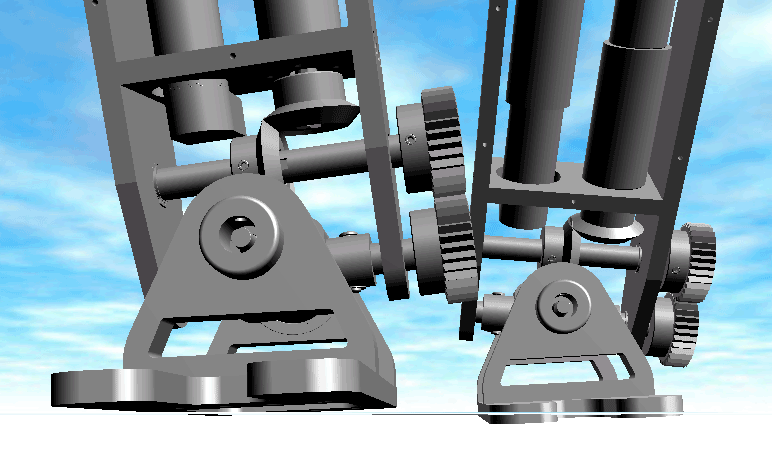
\includegraphics[scale=0.29]{fig/fpe/prestabilization.png}} 
	\subfigure{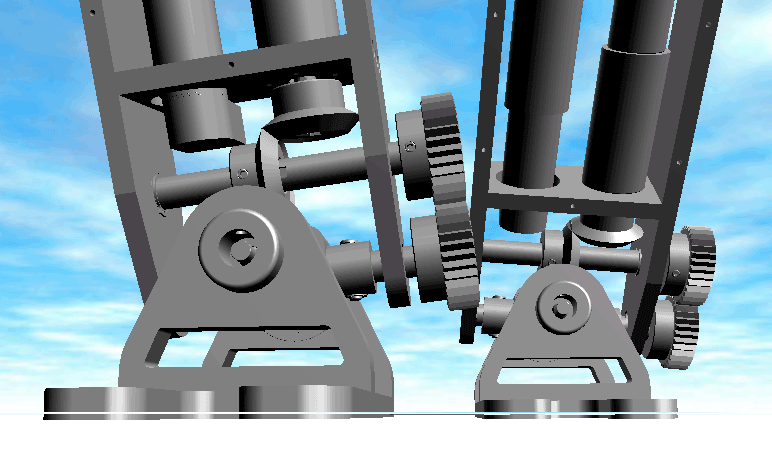
\includegraphics[scale=0.29]{fig/fpe/poststabilization.png}}
	\end{center}
  	\caption{Ground-foot contact shown for before (left) and after (right) contact stabilization.}
	\label{fig:contact_stabilization}
\end{figure}


% subsubsection drop (end)

% subsection joint_level_control (end)

\subsection{Computing FPE Parameters} % (fold)
\label{sub:computing_fpe_parameters}
The 2D FPE equation (\ref{eq:fpe}) requires the total inertia about the COM ($I_{COM}$) and average angular velocity about the pivoted fixed foot ($\dot{\theta}_{avg}$). In the 2D case, the moment of inertia for link $k$ is a scalar value since there is only one plane of rotation. The total inertia about the COM is computed by summing the moment of inertia for each link in the system. However, the moment of inertia for each link is a $3\times3$ tensor: 

\begin{equation}
	\begin{aligned}
		{I_k} = \left[ {\begin{array}{*{20}{c}}
{{I_{xx}}}&{{I_{xy}}}&{{I_{xz}}}\\
{{I_{yx}}}&{{I_{yy}}}&{{I_{yz}}}\\
{{I_{zx}}}&{{I_{zy}}}&{{I_{zz}}}
\end{array}} \right]
	\end{aligned}
\end{equation}

The inertia tensor of each link is taken at the COM aligned with the local coordinate system. If the $xz$-plane is selected as the sagittal plane in 3D space and the moment of inertia of link $k$ is the $I_{yy}$ term. However, in the 3D case the motion of the biped is no longer fixed to a single plane of rotation. By attaching a fixed coordinate frame to the selected sagittal plane at the start of each step, the orientation of the sagittal plane can be expressed as a $3\times3$ rotation matrix $R$. The local inertia tensor can be rotated into the selected sagittal plane's coordinate frame by: 

\begin{equation}
	\begin{aligned}
		{I_{k,sagittal}} = R \cdot {I_k} \cdot {R^T}
	\end{aligned}
	\label{eq:isagittal}
\end{equation}

Then the effective moment of inertia of each link \emph{projected on to the selected sagittal plane} can be obtained by transforming the inertia tensor with (\ref{eq:isagittal}) and pulling out the $I_{yy}$ term, $I_{k,yy}$. The total inertia about the COM can easily be computed by summing the effective inertia of each link on the sagittal plane: 

\begin{equation}
	\begin{aligned}
		{I_{COM}} = \sum\limits_{k = 1}^n {{I_{k,yy}}}
	\end{aligned}
	\label{eq:icom_3d}
\end{equation}

The average angular velocity is computed as a weighted sum of the inertia of each link \cite{Wight:2008ii}. In the 3D case, the same equation is used with the \emph{effective} moment of inertia of each link on the sagittal plane: 

\begin{equation}
	\begin{aligned}
		{\dot \theta _{avg}} = \frac{{\sum\limits_{k = 1}^n {{I_{k,yy}}} {{\dot \theta }_k}}}{{\sum\limits_{k = 1}^n {{I_{k,yy}}} }}
	\end{aligned}
	\label{eq:wavg_3d}
\end{equation}

The angular velocity of each link ${\dot{\theta}_k}$ is obtained by rotating the joint velocity (expressed as a $3\times1$ vector with $\dot{q}_k$ in the row represented by its local axis of rotation) to the fixed frame of the sagittal plane. 

The parameters computed with (\ref{eq:icom_3d}) and (\ref{eq:wavg_3d}) are plugged in to the 2D FPE equation (\ref{eq:fpe}) and the solution ($\phi$) is obtained with a non-linear equation solver. 
% subsection computing_fpe_parameters (end)

% section extension_to_3d (end)

\section{Simulations and Results} % (fold)
\label{sec:simulations_and_results}

The proposed control strategy to extend the FPE theory to 3D was implemented in simulation on a 14 DOF lower body bipedal robot. Each state of the control strategy was implemented in the Matlab/Simulink environment with the multibody dynamics simulation by SimMechanics. Accurate kinematic and dynamic properties of the physical robot were taken directly from the CAD model through the toolchain model generation process (as discussed in Section~\ref{sec:model_generation}). The controller diagram shown in Figure~\ref{fig:fpecontroller} implements the control strategy presented in this section. The subsystems from the outer most loop working inwards are described as follows: 

\begin{figure*}[!b]
	%\centering
    \centerline{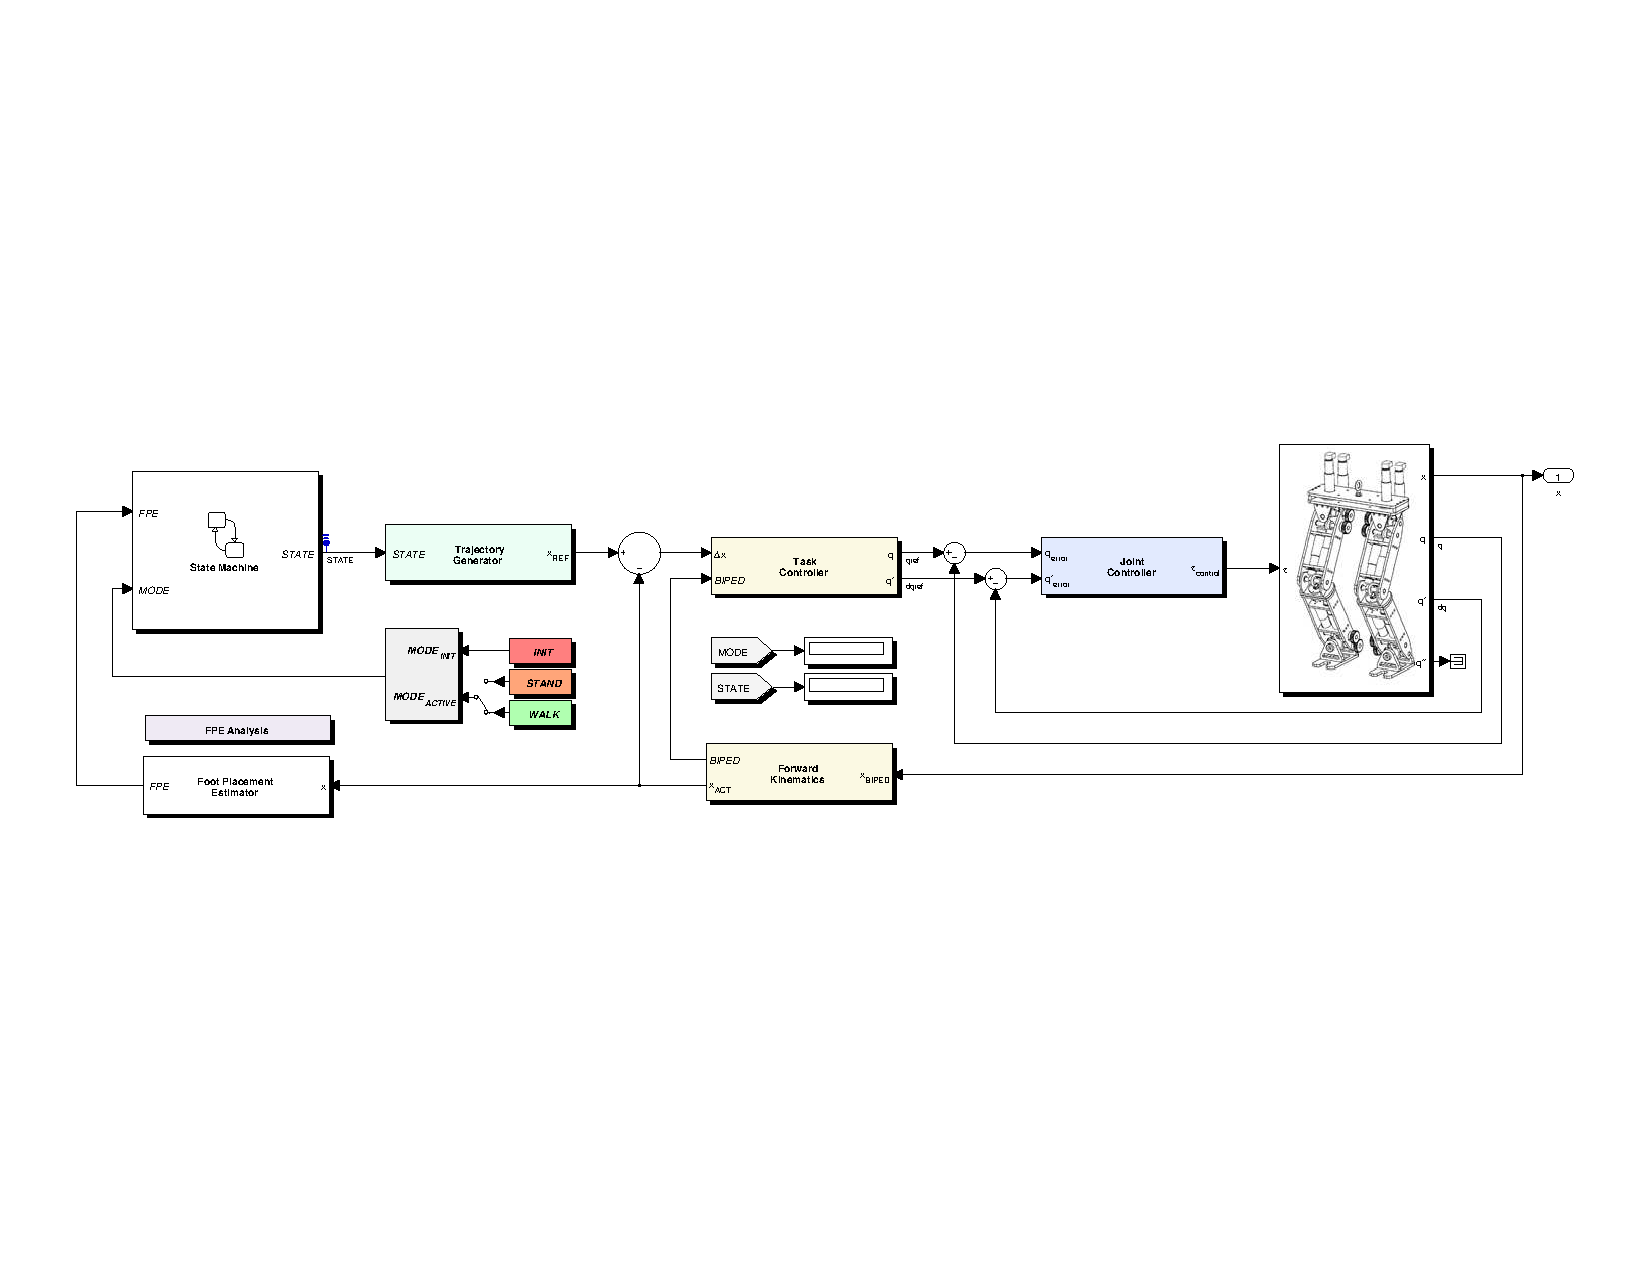
\includegraphics[trim = 12mm 75mm 12mm 75mm,clip,width=18cm]{fig/simulations/fpecontroller.pdf}}
  	\caption{Controller diagram of 3D FPE based walking control strategy implemented in Simulink.}
	\label{fig:fpecontroller}
\end{figure*}

\begin{enumerate}
	\item \textbf{State Machine} \\ 
	Finite state machine logic was implemented in Stateflow as shown in Figure~\ref{fig:stateflow}. The state names follow the same convention as the 2D FPE case (shown in Figure~\ref{fig:statemachine}) while the transition logic is updated for the 3D case described in Section~\ref{sub:joint_level_control}.  \\

	\item \textbf{Trajectory Generator} \\ 
	Generates the task space COM ($x_{COM}$) and the swing foot ($x_{SWING}$) trajectories detailed in Section~\ref{sub:trajectory_generation} based on the current state of the controller. Also uses the higher level supervisory control mode (i.e. \textbf{WALK} or \textbf{STAND}) to adjust the trajectory generation for understepping/overstepping the FPE point. \\

	\item \textbf{Foot Placement Estimator} \\ 
	Computes the FPE parameters about the COM ($I_{COM}$, $\dot{\theta}_{avg}$) for the 3D case (detailed in Section~\ref{sub:computing_fpe_parameters}) and solves the FPE equation (\ref{eq:fpe}) using a numerical methods-based nonlinear solver from \cite{Wight:2008vt}. \\

	\item \textbf{Task Controller} \\ 
	Provides the state dependent control logic for the whole body motion control framework in Section~\ref{sub:control_strategy}. The resulting joint space velocities are integrated to obtain the joint position reference command. The contact stabilization substate used in the second half of \textbf{DROP} is also implemented here to generate joint level trajectories directly. \\

	\item \textbf{Joint Controller} \\ 
	High gain joint level PD controllers with gain scheduling based on the current state of the control strategy. The output of this block ($\tau$) is used to drive the forward dynamics simulation generated with the toolchain. \\

\end{enumerate}

\begin{figure}[!h]
	\centering
    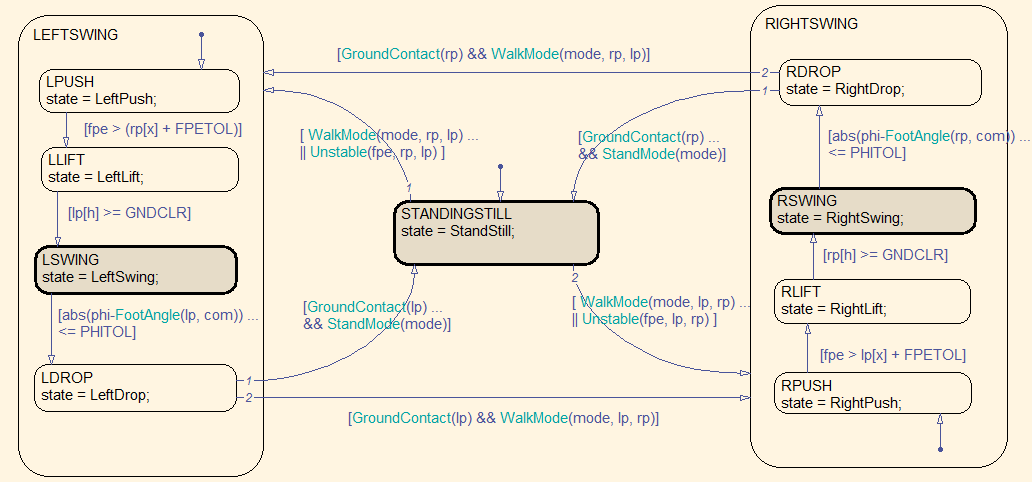
\includegraphics[scale=0.6]{fig/simulations/stateflow.png} 
  	\caption{Finite state machine implemented in Stateflow for 3D FPE-based walking control strategy. \Incomplete}
	\label{fig:stateflow}
\end{figure}

The simulations are executed with a fixed step Runge-Kutta solver at 1KHz. The forward dynamics generated with the toolchain drive the simultaneous 3D visualizations in an external viewer application.  

\subsection{Contact Modeling} % (fold)
\label{sub:full_contact_modeling}
The initial spring-damper contact model discussed in Section~\ref{sub:initial_contact_modeling} was replaced with a more complex version to accurately model the ground/foot dynamics. The Hunt and Crossley contact model \cite{hunt1975coefficient,gilardi2002literature} generates a normal force using a non-linear spring-damper system defined by: 

\begin{equation}
	\label{eq:contacthc}
	{F_{normal}} = b{z^p}{\dot z^q} + k{z^n}
\end{equation}

Where $z$, $\dot{z}$ are the penetration depth position and velocity, respectively. The constants $k$, $b$ are the spring-damper coefficients and $n$, $p$, $q$ are tunable constants. Equation (\ref{eq:contacthc}) provides the ground reaction force in the normal direction only. The tangential (frictional) contact forces were modeled by: 


\begin{equation}
	\label{eq:contactfr}
	{F_{tangential}} = f{\dot x}
\end{equation}

Where $\dot x$ is the tangential velocity of the contact point (in the $x$ and $y$ directions) and $f$ is a tunable constant. The forces generated by (\ref{eq:contacthc}) and (\ref{eq:contactfr}) ensure that there are no discontinuities when ground contact is made. A seperate dynamic simulation model was generated to tune the contact model constants to emulate a stiff ground. The final (tuned) parameters used for dynamic simulations are provided in Table~\ref{tab:contactk}.

\begin{table}[!h]
  \centering
  \caption{Tuned contact model constants.}
    \begin{tabular}{cc}
    \addlinespace
    \toprule
    \textbf{Parameter} & \textbf{Value}\\
    \midrule
	$f$	&	10 \\
    $k$	&	2000 \\
    $b$	&	10 \\
    $p$	&	1.10 \\
    $q$  &	1.00 \\
    $n$	&	2.31 \\
    \bottomrule
    \end{tabular}
  \label{tab:contactk}
\end{table}

It was found that stiffening the ground contact by raising the model constants would produce singularities with fixed time step simulations at 1 KHz. Reducing the time step helped avoid singularities but the simulation runtime drastically increased. The use of variable step solvers was explored as an option to reduce simulation runtime while providing a stiffer ground with much higher contact model constants. 

% subsection contact_modeling (end)

\subsection{Side-to-Side Stepping} % (fold)
\label{sub:3d_simulations}

To demonstrate the dynamic stability of a 3D biped under this approach, the frontal plane was selected as the sagittal plane. Forward motion along this sagittal plane results in a side-to-side stepping sequence for the biped (as shown in Figure \ref{fig:sequence}). The gray plane in the frame captures moves along the Y-direction (biped's frontal plane). The intersection of the gray plane and the ground indicates the FPE point tracked during \textbf{DROP}. 

\begin{figure}[!h]
	\centering
    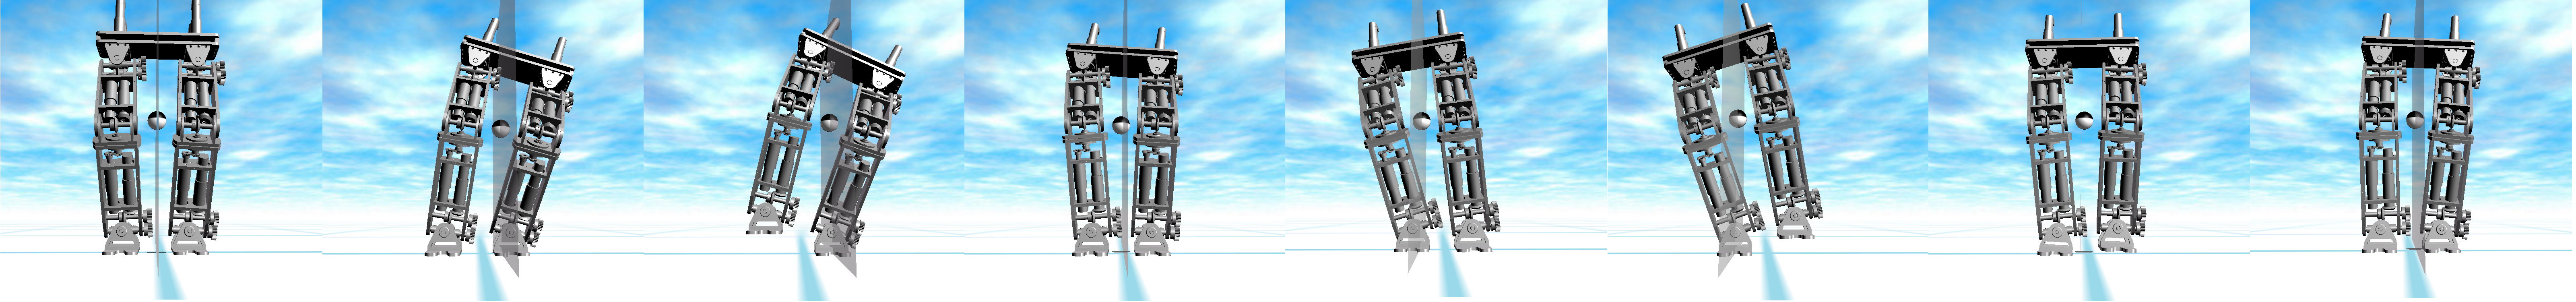
\includegraphics[scale=0.095]{fig/simulations/sequence.png}
  	\caption{Frame captures from the realtime 3D visualization while side-to-side stepping.}
	\label{fig:sequence}
\end{figure}

The resulting $x_{COM}$ trajectories from simulating the side-to-side stepping motion (shown in Figure \ref{fig:comtraj}) demonstrate the stability of the biped through a complete gait sequence. The prioritized motion control framework handles the dynamic switching of constraints (from double support to single support) while generating the appropriate joint level commands for swinging the COM over. The colour coded dotted lines on Figure \ref{fig:comtraj} indicate the boundaries of each foot on the ground. Note that during the \textbf{SWING} state, the COM is pushed outside the region of support (around 11s). This in turn initiates the \textbf{DROP} state where the FPE point is tracked to regain stability.

\begin{figure}[!h]
	\centering
    \includegraphics[scale=0.8]{fig/simulations/comtraj.eps}
  	\caption{COM trajectory being tracked during the complete gait sequence of side stepping.}
	\label{fig:comtraj}
\end{figure}


In the terminal \textbf{DROP} state, the swing foot trajectory tracks the FPE point on the ground (shown in Figure \ref{fig:fpetrack}) with an added offset to ensure that the biped oversteps to guarantee stability (as per the 2D FPE theory). Once ground contact is made (around 11.6s), the stabilization substate is entered and the swing foot trajectory is controlled directly to align the foot with the ground. This causes the biped to rock back and forth (similar to the 2D case) until stability is reached.

\begin{figure}[!h]
	\centering
    \includegraphics[scale=0.8]{fig/simulations/fpetrack.eps}
  	\caption{Swing foot tracks the a point on the ground given by $FPE + FPE_{offset}$ to ensure overstepping.}
	\label{fig:fpetrack}
\end{figure}


\subsection{Forward Walking Gait} % (fold)
\label{sub:forward_walking_gait}
\Incomplete 
% subsection forward_walking_gait (end)

% section simulations_and_results (end)

\section{Summary} % (fold)
\label{sec:simulations_summary}
The impact of the contact points with the ground is modeled using the conservation of angular momentum to determine the regions in the state space where the biped remains stable after ground contact, by analyzing the total system energy post impact. The stability analysis is then used to determine where a biped must step to remain within the stability region. This forms the basis of the FPE, which is a point on the ground where, if the robot were to step onto that point, the kinetic energy of the biped system would equal the peak potential energy. Placing the swing foot beyond the FPE point results in the biped not having enough kinetic energy post impact to overcome the peak potential energy (overstepping). In this case, the biped remains stable. Conversely, placing the swing foot before the FPE point causes the kinetic energy post impact to exceed the peak potential energy (understepping). In this situation the biped begins to fall over.

% section discussion (end)

% chapter simulations (end)